\documentclass{article}%
\usepackage[T1]{fontenc}%
\usepackage[utf8]{inputenc}%
\usepackage{lmodern}%
\usepackage{textcomp}%
\usepackage{lastpage}%
\usepackage[head=40pt,margin=0.5in,bottom=0.6in]{geometry}%
\usepackage{graphicx}%
%
\title{\textbf{Gobierno subió 39.900\% precio de las cajas CLAP y contienen menos productos}}%
\author{CARLOS SEIJAS MENESES | @carlosgmeneses}%
\date{10/10/2018}%
%
\begin{document}%
\normalsize%
\maketitle%
\textbf{URL: }%
http://www.el{-}nacional.com/noticias/economia/gobierno{-}subio{-}39900{-}precio{-}las{-}cajas{-}clap{-}contienen{-}menos{-}productos\_255119\newline%
%
\textbf{Periodico: }%
EN, %
ID: %
255119, %
Seccion: %
Economía\newline%
%
\textbf{Palabras Claves: }%
Economía\newline%
%
\textbf{Derecho: }%
2.10, %
Otros Derechos: %
, %
Sub Derechos: %
2.10.1\newline%
%
\textbf{EP: }%
NO\newline%
\newline%
%
\textbf{\textit{En 2016, 11 alimentos llegaron en la primera entrega que se hizo a las comunidades de Pinto Salinas y Simón Rodríguez. El mes pasado solo recibieron 6}}%
\newline%
\newline%
%
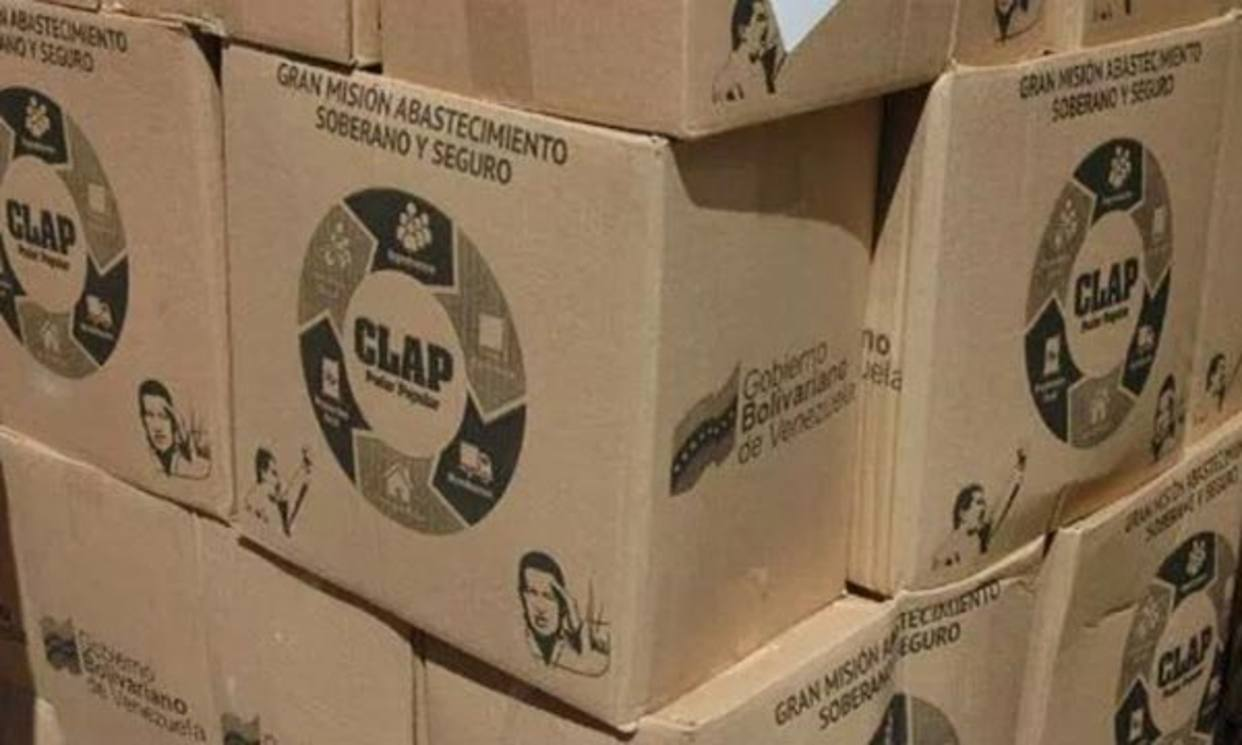
\includegraphics[width=300px]{240.jpg}%
\newline%
%
Vecinos de comunidades de Caracas rechazaron el incremento de 39.900\% ~del precio de las cajas de alimentos de los Comités Locales de Abastecimiento y Producción. Subió de~0,25 a~100 bolívares soberanos. Aseguraron que cada vez traen menos productos y son de muy mala calidad. “El gobierno le aumentó el valor a la miseria de los ciudadanos que no pueden adquirir~todos los alimentos con el salario que perciben”, expresó Ana Mijares, de Pinto Salinas. “Los vecinos coincidimos en que a la gente le da dolor de estómago después de tomar la leche”, afirmó.%
\newline%
%
En un principio hubo dudas sobre el monto que tendrían que cancelar. El 29 de agosto Kendy Graterol, responsable de la mesa de alimentación de Nueva Esparta, informó en rueda de prensa que a partir del 1° de septiembre la caja tendría un precio de 150 bolívares, información que fue ratificada por el coordinador nacional de los CLAP,~Freddy Bernal. Sin embargo, una semana después el funcionario rectificó y anunció que serían 100 bolívares, como dijo el vicepresidente del Área Económica, Tareck el Aissami.%
\newline%
%
Esta semana, residentes de un edificio ubicado en la parroquia Candelaria pagaron 117 bolívares soberanos: 100 por la caja, 10 por el transporte, 5 por la logística y 2 por la papelería. Patricia Jiménez, vecina, afirmó que el contenido es muy deficiente. “Trajo granos (caraotas y lentejas), un atún que no es de la mejor calidad, dos paquetes de leche en polvo, que tiene mucha lactosa y que no es buena para niños pequeños ni para personas que tienen intolerancia a la lactosa”.%
\newline%
%
También señaló que el gobierno insiste en que los beneficiarios tengan el carnet de la patria como requisito para recibir la caja, pero en el edificio, así como en otras comunidades, les han dado un poco de larga al asunto.%
\newline%
%
Los vecinos denuncian irregularidades en la entrega de la caja. Aseguran que a veces llega abierta, con menos productos y que para una familia de cinco miembros los alimentos no alcanzan para más de una semana. Pero siguen pagándola porque trae productos que difícilmente se consiguen en el mercado, como aceite, azúcar y arroz.%
\newline%
%
A una residente de la parroquia~La Vega, sin embargo, no le llegó arroz, leche ni enlatados en la caja que recibió el viernes de la semana pasada. Y le cobraron 100 bolívares.%
\newline%
%
En septiembre de 2016, fecha de la primera entrega del beneficio a la comunidad, llegaron aproximadamente 11 alimentos: 2 kilos de leche, 6 atunes, 2,5 kilos de pasta, un kilo de azúcar,~2 litros~de aceite, 3 kilos de caraotas, 3 de lentejas, mayonesa, salsa de tomate, arroz y harina de maíz precocida.. El mes pasado, solo trajo 6: un kilo de leche, un empaque de~500 gramos~de pasta, 4 kilos de harina mexicana, lentejas, arroz y un litro de aceite.%
\newline%
%
En Ciudad Tiuna, conocida como “Los Chinos”, una vecina, que prefirió no identificarse, aseguró que hay bebés y niños desnutridos por la leche~de mala calidad que le entregan. Dijo que los padres, al no poder pagar la que se consigue en el mercado, se ven forzados a dárselas a sus hijos. Agregó que también es fatal la calidad de la pasta y el arroz.%
\newline%
%
Desde hace nueve meses, Juan Pérez, de Caricuao, recibe mensualmente una bolsa del CLAP. La última vez que le llegó, hace 3 semanas, pagó 0,20 bolívares soberanos. El consejo comunal del sector ya les informó sobre el aumento. “Da lástima recibir la bolsa porque le están sacando los productos. Le sacan un kilo de arroz, uno de azúcar y un litro de aceite”.%
\newline%
%
Contó que antes contenía tres o cuatro empaques del mismo producto, pero lo fueron reduciendo a pesar de que siguieron cobrando el mismo monto. “El gobierno hace lo que quiere. Dicen que el precio no debería aumentar porque es subsidiado, pero como sabemos que el gobierno necesita dinero requiere subir los precios, si no de dónde van a salir los pagos de esos sueldos”, razonó Pérez.%
\newline%
%
\end{document}